\documentclass[simplex.tex]{subfiles}
% NO NEED TO INPUT PREAMBLES HERE
% packages are inherited; you can compile this on its own
\begin{document}
\subsection{Non-Parametric Shape Clustering}
%
We have been mostly focused on developing 
non-parametric clustering methods.
To this purpose, we are exploring ideas from energy statistics,
which is non-parametric,
robust, and rotational invariant, thus it incorporates the main ingredients
that we are looking for. The main difficulty is to formulate an 
algorithm based on this, i.e. to identify the correct test 
statistic, or to formulate it as a feasible optimization problem.
Consider $K$-Means clustering problem which is 
$
\min_{\{\mathcal{C}_k\}} 
\sum_{k=1}^K \sum_{x \in \mathcal{C}_k} \| x - \mu_k  \|^2,
$
where $\mathcal{C}_k$ is the $k$th cluster and $\mu_k$ the mean of its points.
We showed that this problem is equivalent to
\begin{equation}
\max_{G} \textnormal{Tr}\left( G^T K G \right) \qquad 
\mbox{s.t. \, $G \ge 0$, $G^T G=I$, $G G^T e_1 = e_1$}.
\end{equation}
where $e_1 = (1,1,\dotsc,1)^T$.
This is a Quadratically Constrained Quadratic Problem (QCQP), which is usually 
NP-hard.
Analogously, consider the energy function 
$\mathcal{E}(F,G) = 2\mathbb{E} \| X - Y\| - \mathbb{E}\| X - X'\| - \mathbb{E}
\| Y - Y'\|$ between $X,X' \sim F$ and $Y,Y' \sim G$. We showed that this can
be written as $\mathcal{E}(A,B) = e_1^T \Delta e_1 $, where $\Delta$ is a
dissimilarity 
matrix between the two sets of data points 
$A \stackrel{iid}{\sim} F$ 
and $B \stackrel{iid}{\sim} G$.
Consequently, a simple two-class clustering problem would be
\begin{equation}
\max_{x,z\in \mathbb{R}^N} x^T \Delta z \qquad 
\mbox{s.t. $x_i^2=1$, $x+z = 0$},
\end{equation}
which is also a QCQP problem. We are currently investigating this problem and
trying to generalize it correctly for more classes.
A simple check of the energy function as a test statistic 
is shown in Fig.~\ref{fig:nonpar}. 
Under the null $F = G$, 
$T$ converges to a quadratic form of normally distributed random variables. This
seems to be the case in the first (blue) histogram, while it is definitely not
the case in the other (red and green) histograms. 
For the blue histogram a single test gives
$T \approx 0.32$ (small), for the red
histogram $T \approx 4000 $ (large), and for the green 
histogram $T \approx 105$ (large), with
only a few points. Thus, energy statistics based approach is 
able to distinguish between
different distributions, even when the clusters have the same mean, which is a
property that $K$-Means cannot resolve.

%
\begin{figure}[h!]
\begin{cframed}
\centering
%\begin{subfigure}[t]{0.45\textwidth}
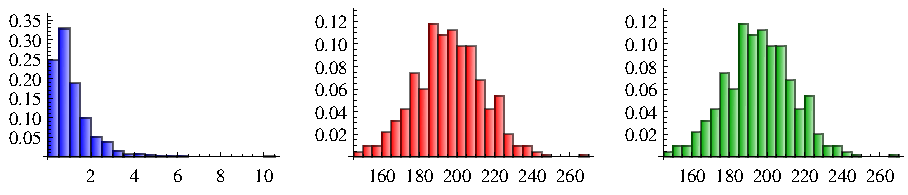
\includegraphics[width=\textwidth]{../../figs/energy_hists.pdf}
%\label{fig:nonpar57}
\caption{
Distribution of test statistic 
$T\equiv\tfrac{n m }{n+m}\mathcal{E}(A,B)$ 
for an ensamble obtained from two distributions:
$A \stackrel{iid}{\sim} \mathcal{N}(\mu_A,\sigma_A^2)$ and
$B \stackrel{iid}{\sim} \mathcal{N}(\mu_B, \sigma_B^2)$, where
$|A|=n$ and $|B|=m$.
Blue histogram: $\mu_A = \mu_B = 0$ and $\sigma_A = \sigma_B = 1$;
Red histogram: $\mu_A = - \mu_B = 1$ and $\sigma_A = \sigma_B = 1$;
Green histogram: $\mu_A = \mu_B = 0$, $\sigma_A = 1$ and $\sigma_B = 1.5$.
}
%\end{subfigure}
%\begin{subfigure}[t]{0.45\textwidth}
%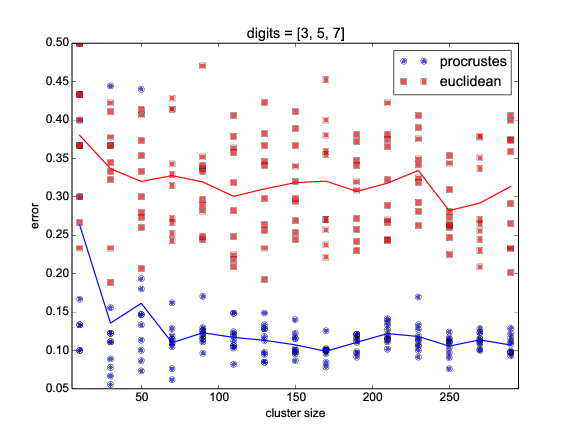
\includegraphics[width=\textwidth]{../../figs/nonPar357.png}
%\label{fig:nonpar357}
%\caption{
%Classification error against the size of each
%cluster (the three classes have the same number of points) is
%shown in blue. The red line is standard
%K-means with Euclidean distance for comparison.}
%\end{subfigure}
%\caption{
%  MNIST handwritten digits and classification error results.
%}
\label{fig:nonpar}
\end{cframed}
\end{figure}
%
\end{document}
